\chapter{Законы сохранения для различных динамических характеристик атмосферы}
Для изучения атмосферных процессов часто удобнее использовать уравнения сохранения не для исходных переменных (компонентов скорости), а для некоторых характеристик, причем таких, которые сохранялись бы в движущейся частице. Такие новые переменные называются инвариантами, т.к. они в движущейся частице сохраняются. Термодинамические адиабатические инварианты -- энтропия, потенциальная температура, псевдо-потенциальная температура получили широкое распространение в 20-е -- 30-е годы прошлого столетия. Адиабатические инварианты динамического характера начали изучаться позднее. Сюда относятся в прежде всего понятия вихря и потенциального вихря. Первый из них является инвариантом лишь в случае плоского течения и несжимаемой жидкости, второй является инвариантом даже в условиях сжимаемой атмосферы. В анализе используются также уравнения сохранения энергии и ряд других уравнений. Выводам этих уравнений и будет посвящена настоящая глава. Все они достаточно широко используются для диагностики моделируемых течений и лучшего понимания механизма образования различных атмосферных циркуляций. 

Вывод соответствующих уравнений будет сделан в декартовой системе координат. В отдельных случаях будут даны их выражения в других системах, но уже без подробного вывода. Поскольку вязкие члены всегда действуют одинаково: способствуют затуханию циркуляции или энергии, мы будем рассматривать для простоты случай идеальной жидкости и иметь дело со следующей системой:

    \begin{align}
        \fd{u} = -\alpha\pd{p}{x}+fv  \label{eq:ch10-DuDt} \\
        \fd{v} = -\alpha\pd{p}{y}-fu \label{eq:ch10-DvDt}  \\
        \fd{w} = -\alpha\pd{p}{z}-g \label{eq:ch10-DzDt}  
    \end{align}
Здесь $\alpha=\frac{1}{\rho}$ -- удельный объем жидкости (газа). Он в данном случае удобнее, чем плотность, т.к. дает более простые выражения при применении операторов дифференцирования. 

\section{{\color{done}Уравнение завихренности}} \label{ch10.1}
Наблюдая за каким-либо объектом в движущийся жидкости или газе мы часто можем заметить, что в движении присутствует вращательный компонент. Если бросить палку в речку, то можно заметить, что она не просто переносится потоком, а совершает одновременно вращательные движение. Это значит, что жидкие частицы, действующие на палку, имеют вращательный компонент. В атмосфере мы непосредственно наблюдаем вращение в мелких вихрях, если частицы воздуха вовлекают в свою циркуляцию какие-нибудь легкие частицы: листья или снежинки. В более крупном масштабе мы можем наблюдать вращательные движения по полю облачности или радиолокационного эха в атмосферных вихрях различного масштаба: тропических и внетропических циклонах. 

В атмосфере вращение частиц происходит частично вследствие термодинамического возбуждения и частично под действием вращения Земли. При изучении динамики атмосферы бывает полезно понять, каким образом генерируется вихревой компонент в движении частицы. При изучении кинематики жидкости было показано, что вектор скорости может быть представлен в виде ряда компонентов: дивергентного, вихревого, трансляционного и деформационного. Ротационный компонент скорости играет в этом ансамбле заметную роль. Идея вывода уравнения вихря состоит в том, чтобы понять, под действием каких процессов может увеличиваться (или убывать) завихренность в движущийся частице или в фиксированной точке пространства и сделать вывод о том, например, усилится циклоническая или антициклоническая циркуляция. Наиболее часть в задачах метеорологии оперируют с вертикальной составляющей завихренности, однако для более полного понимания процесса, лучше рассмотреть компоненты завихренности по всем координатам. Это связано с тем, что горизонтальная завихренность может переходить в вертикальную и наоборот. Кроме того, получив покомпонентные уравнения для завихренности легче понять векторную форму ее записи. Для атмосферы мы можем написать уравнения для относительной и абсолютной завихренности. Начнем с вывода уравнений относительной завихренности.

\begin{warn}
    Абзац ниже нужно слинковать с 1 и 2 главой, где будет говориться о завихренности в базовом (дифференциальном) смысле.
\end{warn}

Как отмечалось в главах \ref{ch1} и \ref{ch2} ({\color{red} ссылки на уравнения завихренности в их базовой форме}) завихренность вдоль осей $Ox$, $Oy$ и $Oz$ имеет следующий вид:
\begin{equation}
    \omega_x = \pd{w}{y}-\pd{v}{z}; \:\: \omega_y = \pd{u}{z}-\pd{w}{x}; \:\:\omega_z = \pd{v}{x}-\pd{u}{y}.
\end{equation}

Начнем последовательно вывод уравнений компонентов завихренности по всем осям. Для получения эволюционного уравнения для компонента $\omega_x$ нужно в левой части результирующего уравнения иметь слагаемое $\td{\omega_x}{t}$. Применим к уравнению (\ref{eq:ch10-DvDt}) оператор $-\pd{}{z}$, а к уравнению $\ref{eq:ch10-DzDt}$ оператор $\pd{}{y}$, будем иметь
\begin{align*}
    -&\pd{}{t}\pd{v}{z}-\pd{u}{z}\pd{v}{x}-u\pd{}{x}\pd{v}{z}-\pd{v}{z}\pd{v}{y} - 
    v\pd{}{y}\pd{v}{z}-\pd{w}{z}\pd{v}{z}-w\pd{}{z}\pd{v}{z} = 
    \pd{\alpha}{z}\pd{p}{y}+\alpha\frac{\partial^2p}{\partial y \partial z} + f\pd{u}{z} \\
    &\pd{}{t}\pd{w}{y}+\pd{u}{y}\pd{w}{x}+u\pd{}{x}\pd{w}{y}+\pd{v}{y}\pd{w}{y} +
    v\pd{}{y}\pd{w}{y}+\pd{w}{y}\pd{w}{z}+w\pd{}{z}\pd{w}{y} = 
    -\pd{\alpha}{y}\pd{p}{z}-\alpha\frac{\partial^2p}{\partial y \partial z} 
\end{align*}
Складывая и группируя члены этих уравнений, получаем
\begin{warn}
    исправить наблу (+u):
\end{warn}

\begin{equation*}
    \td{\omega_x}{t}+\omega_x(\nabla_{yz})-\pd{u}{z}\pd{v}{x}+\pd{u}{y}\pd{w}{x} = \left( \pd{\alpha}{z}\pd{p}{y} - \pd{\alpha}{y}\pd{p}{z} \right) + f\pd{u}{z},
\end{equation*}
здесь $\nabla_{yz} = \pd{v}{y} +\pd{w}{z}$ -- дивергенция в плоскости $yx$. 
Добавляя и вычитая в левой части $\pd{u}{z}\pd{u}{y}$, получим
\begin{equation*}
    -\pd{u}{z}\pd{v}{x}+\pd{u}{y}\pd{w}{x}+\pd{u}{z}\pd{u}{y}-\pd{u}{z}\pd{u}{y} = -\pd{u}{z} \left( \pd{v}{x}-\pd{u}{y} \right) - \pd{u}{y} \left( \pd{u}{z} - \pd{w}{x} \right).
\end{equation*}
Перенося часть членов из левой част ив правую, получаем
\begin{equation*}
    \td{\omega_x}{t} = -\omega_x(\nabla_{yz}) + \omega_z\pd{u}{z}+\omega_y\pd{u}{y}+f\pd{u}{z}+ \left( \pd{\alpha}{z}\pd{p}{y} - \pd{\alpha}{y}\pd{p}{z} \right)
\end{equation*}
или, окончательно,
\begin{equation}
\label{eq:ch10_omegax}
    \td{\omega_x}{t}=
    \underbrace{(\omega_z+f)\pd{u}{z} + \omega_y\pd{u}{y}}_{1}
    \underbrace{\vphantom{(\omega_z+f)\pd{u}{z} + \omega_y\pd{u}{y}}-\omega_x\nabla_{yz}}_{2}+
    \underbrace{\left( \pd{\alpha}{z}\pd{p}{y} - \pd{\alpha}{y}\pd{p}{z} \right)}_{3}
\end{equation}

Для получения эволюционного уравнения $y$-компоненты завихренности $\omega_y$ применим к уравнению (\ref{eq:ch10-DuDt}) оператор $\pd{}{z}$, а к уравнению \ref{eq:ch10-DzDt} оператор $-\pd{}{x}$

\begin{align*}
    &\pd{}{t}\pd{u}{z}+\pd{u}{z}\pd{u}{x}+u\pd{}{x}\pd{u}{z}+\pd{v}{z}\pd{u}{y} + 
    v\pd{}{y}\pd{u}{z}+\pd{w}{z}\pd{u}{z}+w\pd{}{z}\pd{u}{z} = 
    -\pd{\alpha}{z}\pd{p}{x}-\alpha\frac{\partial^2p}{\partial x \partial z} + f\pd{v}{z} \\
    -&\pd{}{t}\pd{w}{x}-\pd{u}{x}\pd{w}{y}-u\pd{}{y}\pd{w}{x}-\pd{v}{x}\pd{w}{y} -
    v\pd{}{y}\pd{w}{x}-\pd{w}{x}\pd{w}{z}-w\pd{}{z}\pd{w}{x} = 
    \pd{\alpha}{x}\pd{p}{z}+\alpha\frac{\partial^2p}{\partial x \partial z} 
\end{align*}
Складывая эти уравнения и группируя члены, получаем
\begin{equation*}
    \td{\omega_y}{t}+\omega_y(\nabla_{xz})+\pd{v}{z}\pd{u}{y}-\pd{v}{x}\pd{w}{y} = \left( \pd{\alpha}{x}\pd{p}{z} - \pd{\alpha}{z}\pd{p}{x} \right) + f\pd{v}{z},
\end{equation*}
здесь $\nabla_{xz} = \pd{u}{x} +\pd{w}{z}$ -- дивергенция в плоскости $xz$. 
Добавляя и вычитая в левой части этого уравнения $\pd{v}{z}\pd{v}{x}$, будем иметь
\begin{equation*}
    -\pd{v}{z}\pd{u}{y}-\pd{v}{x}\pd{w}{y}+\pd{v}{z}\pd{v}{x}-\pd{v}{z}\pd{v}{x} = -\pd{v}{z} \omega_z - \pd{v}{x} \omega_x.
\end{equation*}
Группируя дополнительно члены и перенося часть их них в правую часть уравнения, получим окончательно
\begin{equation}
\label{eq:ch10_omegay}
    \td{\omega_y}{t}=
    \underbrace{(\omega_z+f)\pd{v}{z} + \omega_x\pd{v}{x}}_{1}
    \underbrace{\vphantom{(\omega_z+f)\pd{v}{z} + \omega_x\pd{v}{x}}-\omega_y\nabla_{xz}}_{2}+
    \underbrace{\left( \pd{\alpha}{x}\pd{p}{z} - \pd{\alpha}{z}\pd{p}{x} \right)}_{3}.
\end{equation}

Для получения эволюционного уравнения для вертикальной компоненты завихренности $\omega_z = \pd{u}{x}=\pd{v}{y}$ применим к уравнению (\ref{eq:ch10-DuDt}) оператор $-\pd{}{y}$, а к уравнению (\ref{eq:ch10-DvDt}) оператор $\pd{}{x}$ 
\begin{align*}
    -&\pd{}{t}\pd{u}{y}-\pd{u}{y}\pd{u}{x}-u\pd{}{x}\pd{u}{y}-\pd{v}{y}\pd{u}{y} - 
    v\pd{}{y}\pd{u}{y}-\pd{w}{y}\pd{u}{z}-w\pd{}{z}\pd{u}{y} = 
    \pd{\alpha}{y}\pd{p}{x}+\alpha\frac{\partial^2p}{\partial x \partial y} - \pd{f}{y}v - f\pd{v}{y} \\
    &\pd{}{t}\pd{v}{x}+\pd{u}{x}\pd{v}{x}+u\pd{}{x}\pd{v}{x}+\pd{v}{x}\pd{v}{y} +
    v\pd{}{y}\pd{v}{x}+\pd{w}{x}\pd{v}{z}+w\pd{}{z}\pd{v}{x} = 
    -\pd{\alpha}{x}\pd{p}{y}-\alpha\frac{\partial^2p}{\partial x \partial y} - \cancelto{0}{\pd{f}{x}u} - f\pd{u}{x} \\
\end{align*}
Складывая эти уравнения и группируя члены, получаем
\begin{equation*}
    \td{\omega_z}{t}+\omega_z(\nabla_{xy})-\pd{w}{y}\pd{u}{z}+\pd{w}{x}\pd{v}{y} = \left( \pd{\alpha}{y}\pd{p}{x} - \pd{\alpha}{x}\pd{p}{y} \right) - f\nabla_{xy} - \beta v,
\end{equation*}
здесь $\nabla_{xy}=\pd{u}{x}+\pd{v}{y}$ -- дивергенция в плоскости $xy$. Добавляя и вычитая $\left( \pd{w}{x}\pd{w}{y} \right)$, будем иметь
\begin{equation*}
    -\pd{w}{y}\pd{u}{z}+\pd{w}{x}\pd{v}{y}+\pd{w}{x}\pd{w}{y}-\pd{w}{x}\pd{w}{y} = 
    -\pd{w}{x} \underbrace{ \left( \pd{w}{y} - \pd{v}{z} \right) }_{\omega_x} 
    -\pd{w}{y} \underbrace{ \left( \pd{u}{z} - \pd{w}{x} \right) }_{\omega_y} 
\end{equation*}
Группируя дополнительно члены и перенося часть их них в правую часть уравнения, получим окончательно
\begin{equation}
\label{eq:ch10_omegaz}
    \td{\omega_z}{t}=
    \underbrace{\omega_x\pd{w}{x} + \omega_y\pd{w}{y} -\beta v }_{1} - 
    \underbrace{\vphantom{(\omega_z+f)\pd{v}{z} + \omega_x\pd{v}{x}}
    \left( \omega_z + f \right) \nabla_{xy}}_{2}+
    \underbrace{\left( \pd{\alpha}{y}\pd{p}{x} - \pd{\alpha}{x}\pd{p}{y} \right)}_{3}.
\end{equation}

Из этого и аналогичных уравнений для $\omega_x$ и $\omega_y$ видно, что индивидуальная скорость изменения относительной завихренности зависит от трех групп членов, каждую их которых можно рассматривать как завихренность вокруг соответствующей оси. Рассмотрим конкретно вертикальный компонент завихренности, а к сравнению разных компонент завихренности придем позже. 

Первую группу слагаемых (три первых слагаемых в правой части уравнения \ref{eq:ch10_omegaz}) называют по-разному: эффектом вихревой трубки, членом наклона завихренности (tilting) или членом закручивания (twisting). Эти члены характеризуют превращение завихренности по двум другим осям в завихренность вдоль данной оси. В случае $\omega_z$ происходит переход двух горизонтальных компонент в вертикальную, т.е. горизонтальные вихревые трубки как бы наклоняются, именно поэтому поэтому члены и называются членами наклона. 

    \begin{figure}[h]
    \centering
    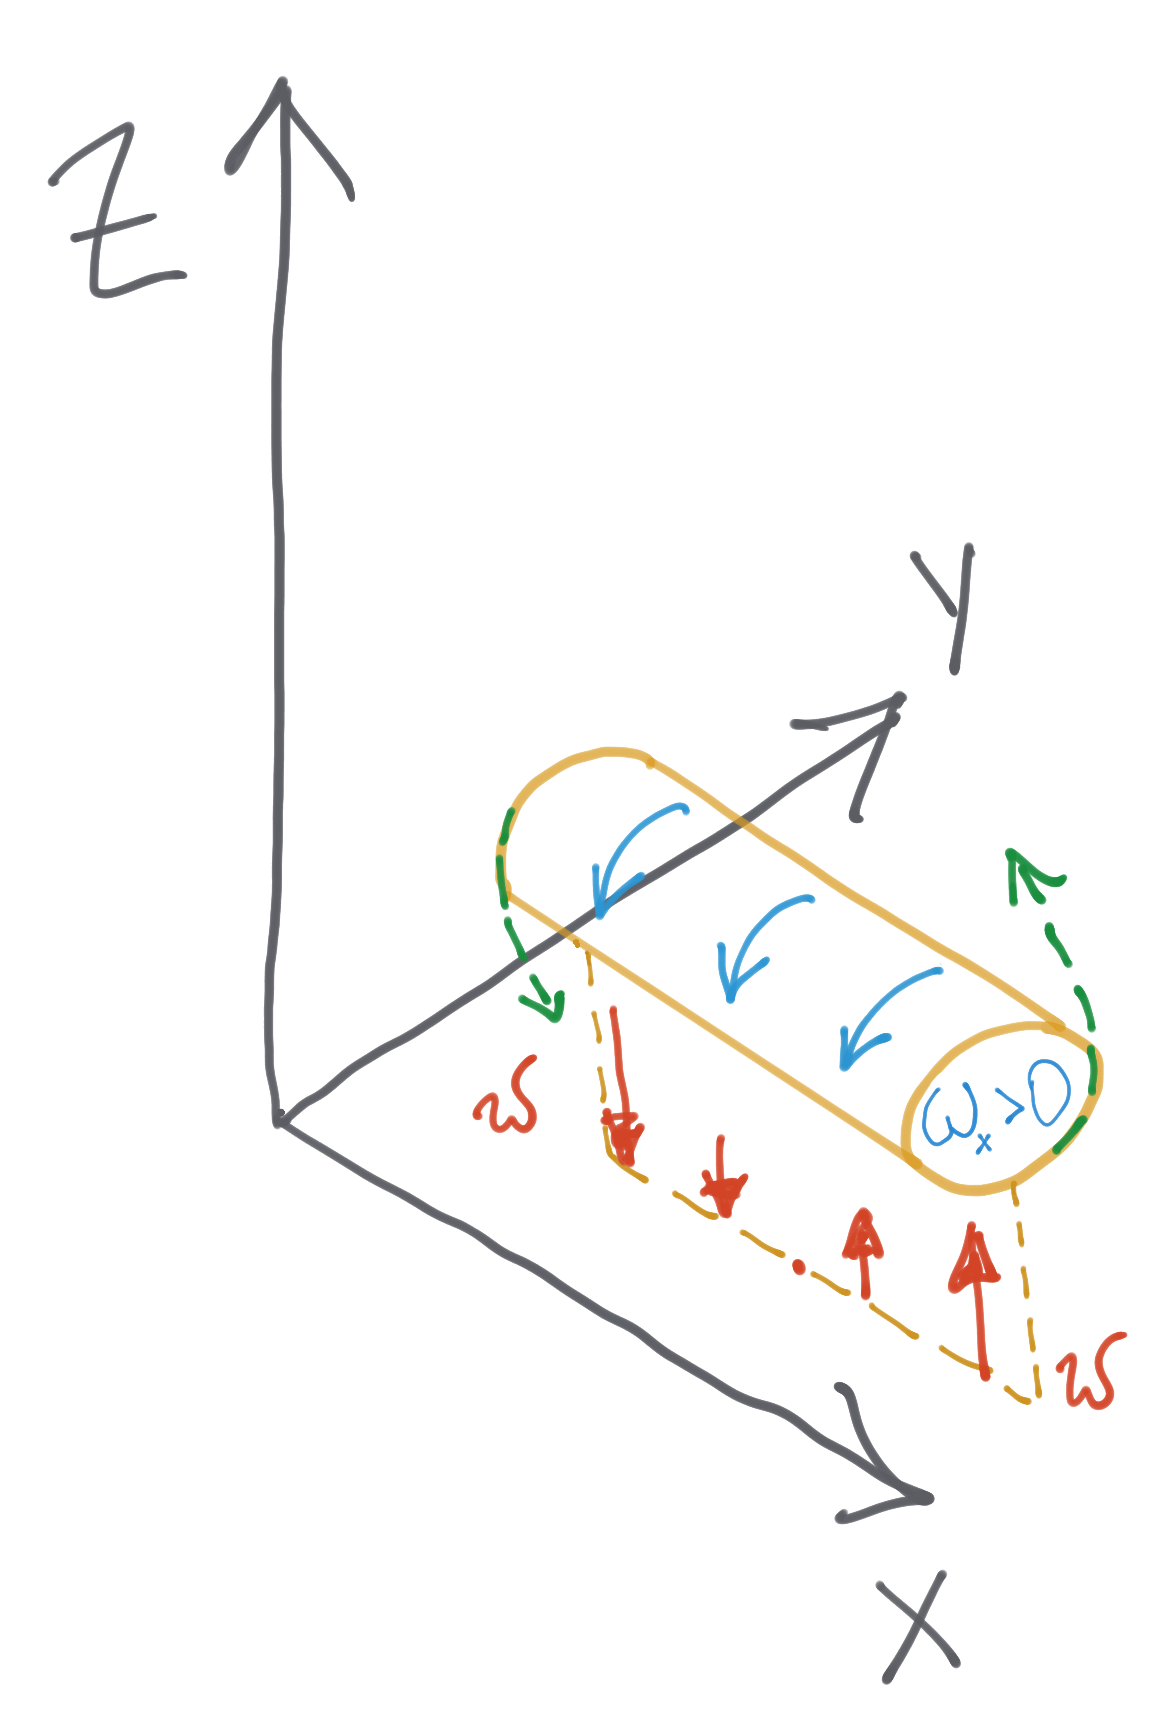
\includegraphics[width=0.5\linewidth]{pics/ch10.1.png}
    \caption{\label{fig:ch10.1}
    Пояснение условия члена наклона на примере действия члена $\omega_x\pd{w}{x}$
    }
    \end{figure}    

Поясним действие члена наклона на примере действия члена $\omega_x\pd{w}{x}$. Пусть для определенности $\omega_x > 0$, то есть вращение происходит против часовой стрелки и пусть распределение вертикальной скорости таково, что $\pd{w}{x}>0$ (красные стрелки на рисунке \ref{fig:ch10.1}). Тогда материальная кривая, образующая цилиндр и находящаяся первоначально в вертикальной плоскости $zOy$ и вдоль которой циркулирует воздух вокруг оси $Ox$, будет наклоняться вертикальными движениями так, как это показано пунктирными зелеными стрелками, и приведет к тому, что будет увеличиваться завихренность в вертикальном направлении $\left( \td{\omega_z}{t}>0 \right)$. Этот эффект существенен, так как позволяет переводить довольно большие значения $\omega_x$ и $\omega_y$ в $\omega_z$. 
\begin{warn}
    В рукописях (дополнение к стр 4) есть еще аналог масштабного анализа для одного частного случай. Я не уверен, что это нужно сюда вставлять.
\end{warn}
Если рассматриваются движения большого масштаба, то генерация завихренности может происходить также под действием $\beta$-эффекта. Необходимо отметить, что эта группа членов является источником и стоком завихренности.

Вторая группа членов (четвертое слагаемое в уравнении (\ref{eq:ch10_omegaz})) характеризует влияние дивергенции в плоскости, нормальной к компоненту завихренности, на усиление или ослабление завихренности. Эти члены оказывают воздействие только в том случае, когда завихренность уже существует. 

Так как $\nabla_{xy}<0$ характеризует конвергенцию, то в этом случае уже существующая положительная завихренность усиливается (вихревая трубка сужается и циркуляция в ней становится сильнее), а в случае дивергенции -- ослабевает (вихревая трубка расширяется). Этот член часто называют членом вытягивания (stretching), поскольку он вытягивает вихревую трубку. 
    \begin{figure}[h]
    \centering
    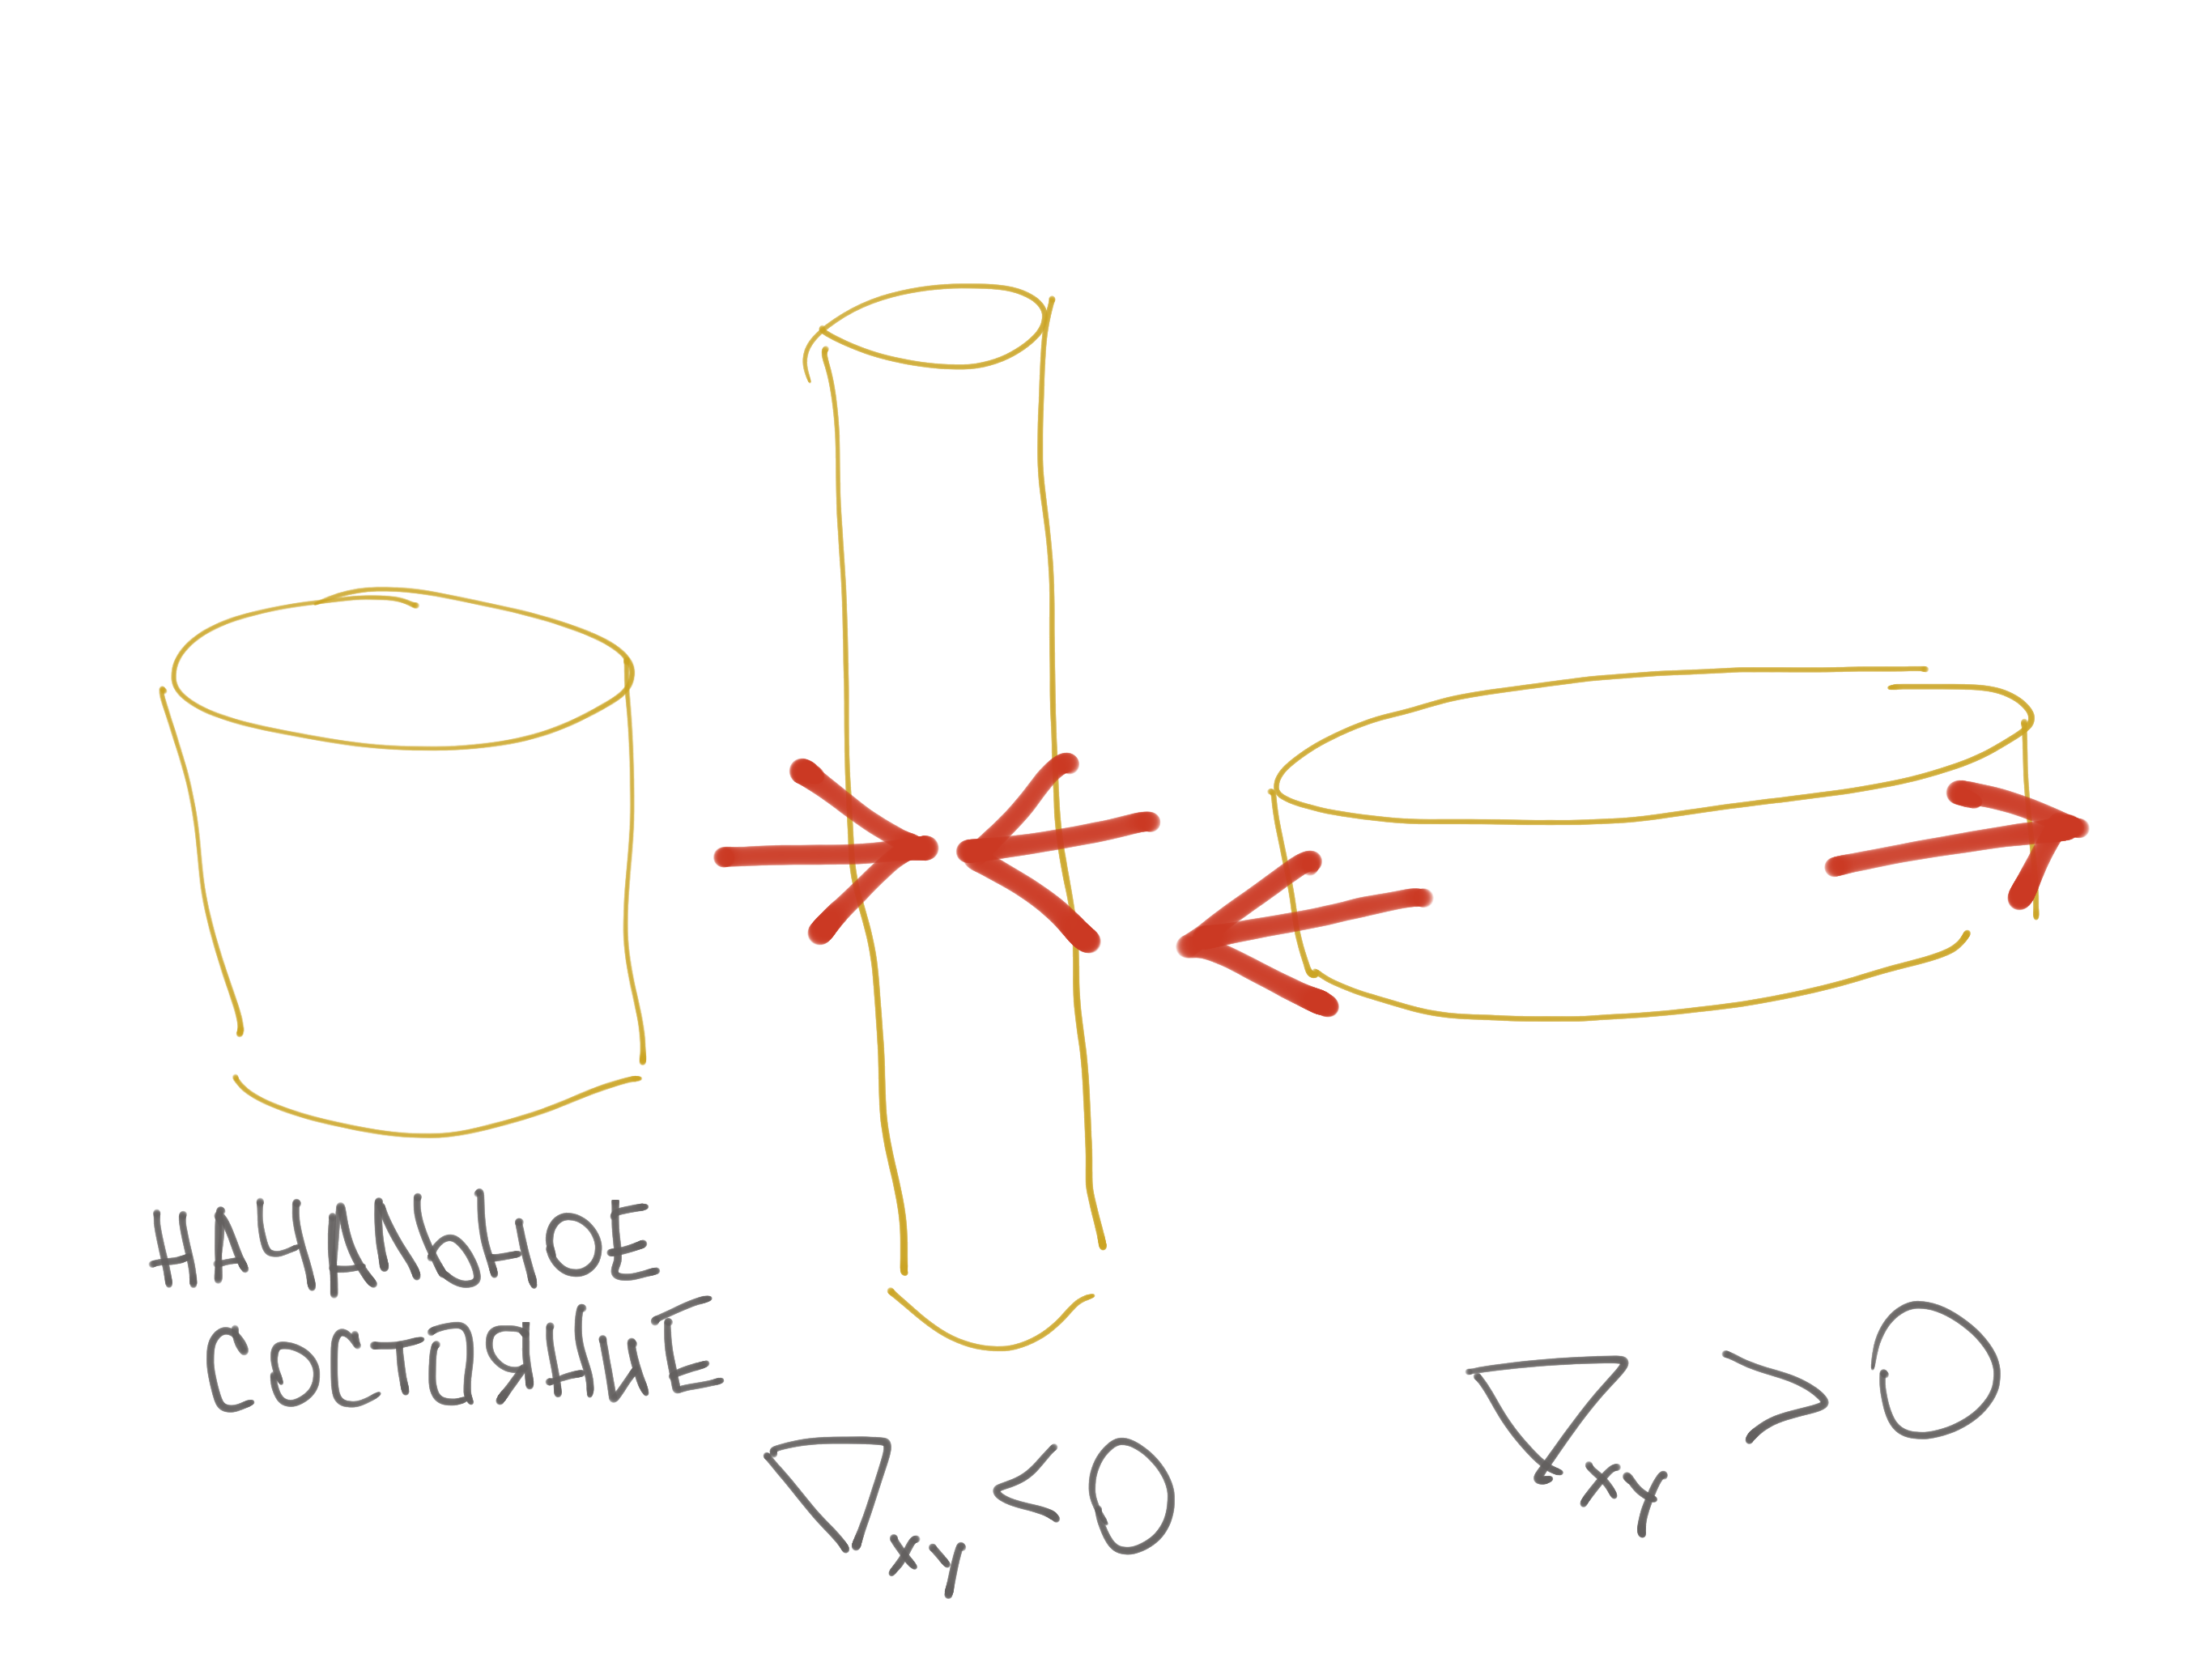
\includegraphics[width=0.5\linewidth]{pics/ch10.2.png}
    \caption{\label{fig:ch10.2}
    Пояснение условия члена вытягивания
    }
    \end{figure}    
Вертикальное вытягивание колонки воздуха увеличивает его завихренность. Процесс здесь подобен тому, который можно наблюдать у фигуристов. Сначала они раскручиваются с расставленными руками, а затем прижимают их к телу много усиливая скорость вращения. При необходимости замедлить вращение руки снова открываются. Прижимание и открытие рук подобно действию конвергенции и дивергенции, соответственно. 

Последних два слагаемывх в уварнении (\ref{eq:ch10_omegaz}) описывают завихренность за счет бароклинности. Предствим их в векторной форме:

\begin{equation*}
    \pd{\alpha}{y}\pd{p}{x}-\pd{\alpha}{x}\pd{p}{y}=\vec{k} \left( \nabla_hp \times \nabla_h\alpha \right) = \vec{k} \left( \nabla_hp \times \nabla_hT \right) \frac{R}{\rho}  
\end{equation*}
{\color{red}Вывод этой формулы будет сделан несколько позднее.} Графически действие этого члена представлено так: 
    \begin{figure}[h]
    \centering
    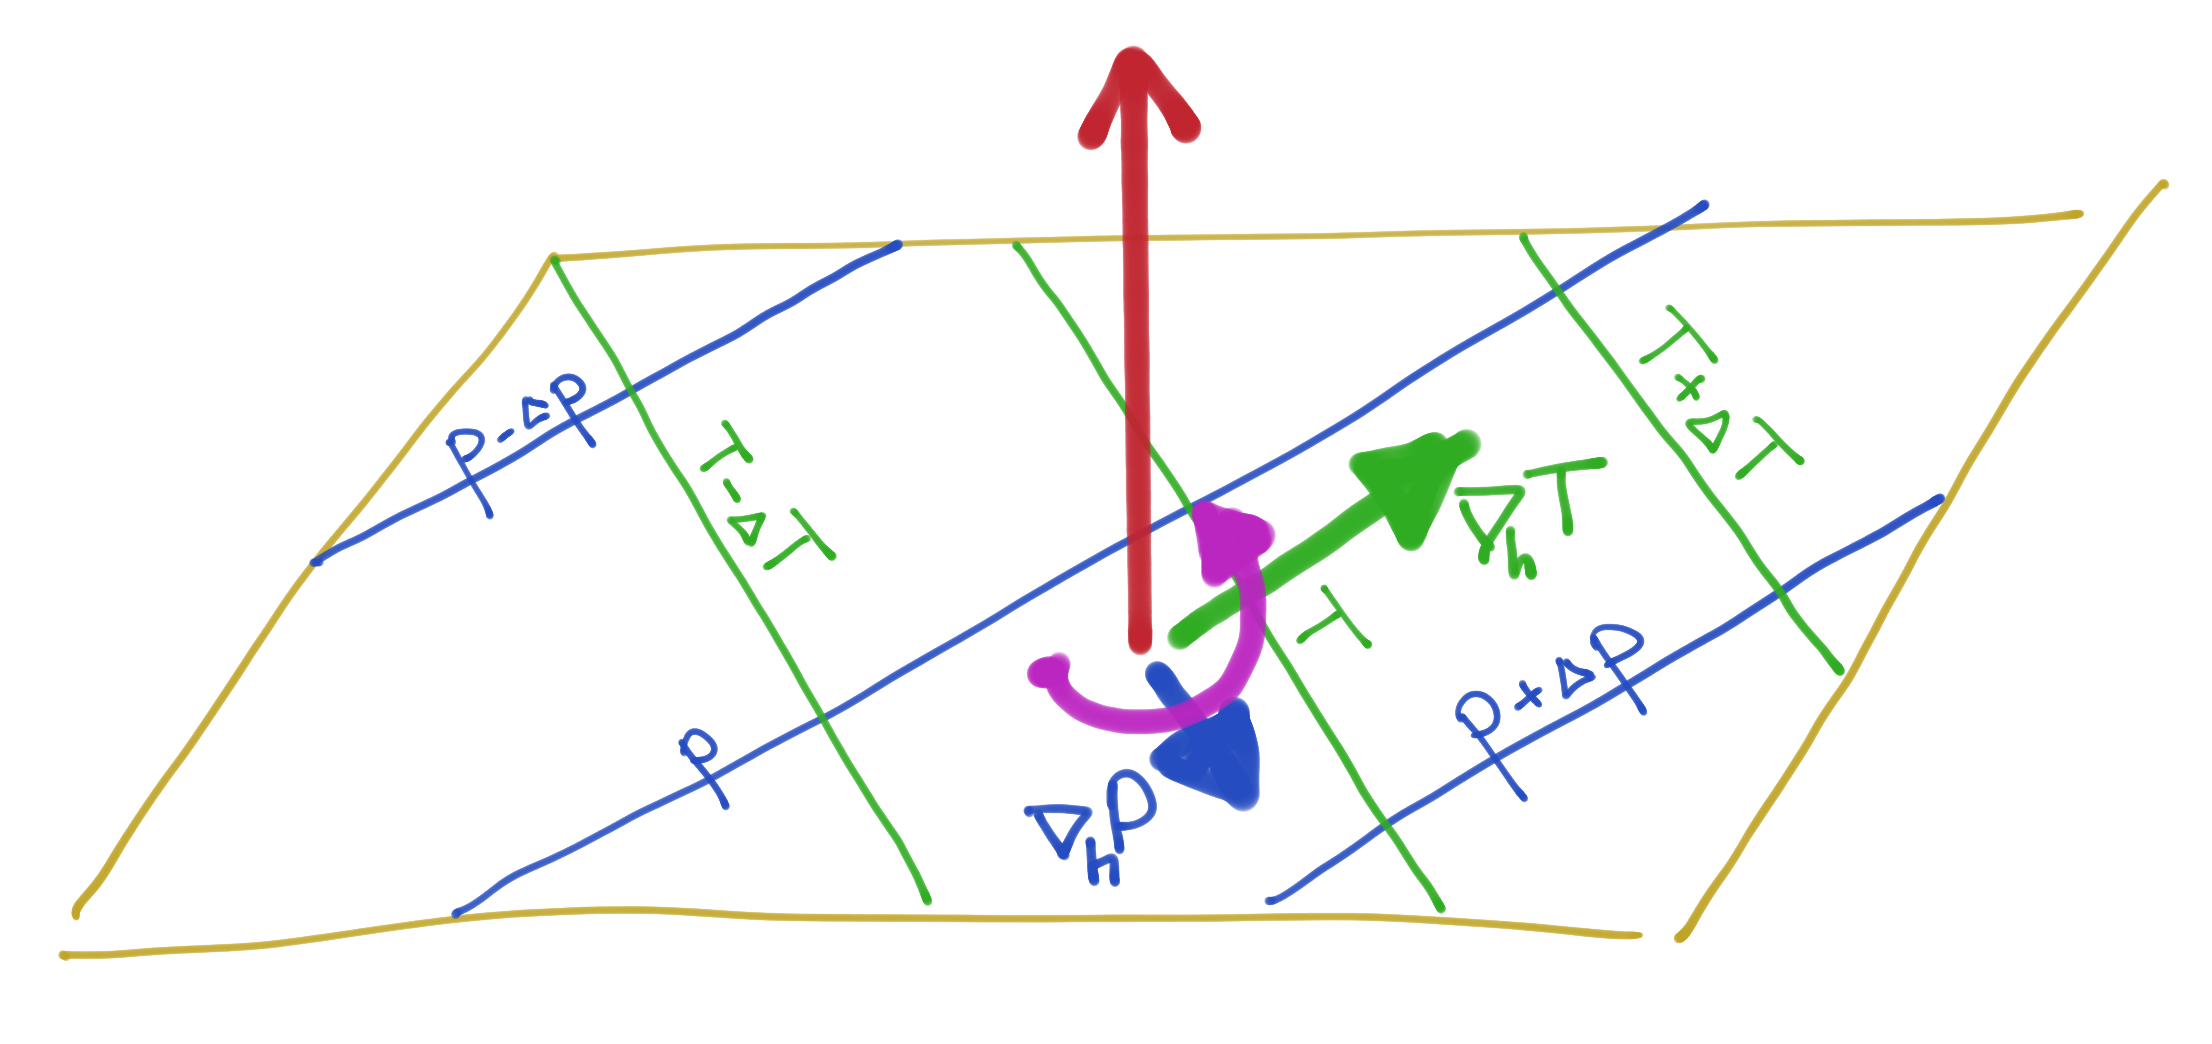
\includegraphics[width=0.9\linewidth]{pics/ch10.3.png}
    \caption{\label{fig:ch10.3}
    Пояснение действия члена бароклинности
    }
    \end{figure}    
Здесь $\nabla_h$ обозначает оператор горизонтального градиента. При направлении градиентов давления и температуры, изображенном на этом рисунке завихренность должна быть положительной и циркуляция происходить в направлении от конца вектора $\nabla_hp$ к концу вектора $\nabla_hT$ в направлении {\color{red}меньшего угла между ними} как это показано розовой стрелкой на рисунке \ref{fig:ch10.3}. 

Запишем теперь полученные нами уравнения для компонентов вихря более единообразно. Наши исходные компоненты завихренности имеют вид
\begin{align}
    \td{\omega_x}{t}&= (\omega_z+f)\pd{u}{z} + \omega_y\pd{u}{y}
    -\omega_x\nabla_{yz}+\left( \pd{\alpha}{z}\pd{p}{y} - \pd{\alpha}{y}\pd{p}{z} \right) \label{eq:ch10_omegax1} \\
    \td{\omega_y}{t}&=(\omega_z+f)\pd{v}{z} + \omega_x\pd{v}{x}
    -\omega_y\nabla_{xz}+\left( \pd{\alpha}{x}\pd{p}{z} - \pd{\alpha}{z}\pd{p}{x} \right) \label{eq:ch10_omegay1} \\
    \td{\omega_z}{t}&=
    \omega_x\pd{w}{x} + \omega_y\pd{w}{y} -\beta v - 
    \left( \omega_z + f \right) \nabla_{xy}+
    \left( \pd{\alpha}{y}\pd{p}{x} - \pd{\alpha}{x}\pd{p}{y} \right) \label{eq:ch10_omegaz1}.
\end{align}
Глядя на эти уравнения можно заметить, что имеется некоторая асимметрия в появлении силы Кориолиса в разных уравнениях. Это связано с тем, что не все компоненты ускорения силы Кориолиса были учтены в исходных уравнениях движения, а также с тем, что учитывалось только его изменение вдоль оси $y$. 

Чтобы сделать уравнения (\ref{eq:ch10_omegax1})-(\ref{eq:ch10_omegaz1}) более единообразными, прибавим и вычтем в каждом уравнении члены, которые превратят разные плоские дивергенции в полную дивергенцию в каждом уравнении. Добавляя и вычитая в правой части уравнения (\ref{eq:ch10_omegax1}) член $\omega_x\pd{u}{x}$, в уравнении (\ref{eq:ch10_omegay1}) $\omega_y\pd{v}{y}$, а в уравнении (\ref{eq:ch10_omegaz1}) $\omega_z\pd{w}{z}$, получим 

\begin{align}
    \td{\omega_x}{t}&= \omega_x\pd{u}{x} + \omega_y\pd{u}{y} + (\omega_z+f)\pd{u}{z} - \omega_x\nabla\vec{u}-\left( \pd{\alpha}{y}\pd{p}{z} - \pd{\alpha}{z}\pd{p}{y} \right) \label{eq:ch10_omegax2} \\
    \td{\omega_y}{t}&=\omega_y\pd{v}{y} + \omega_x\pd{v}{x} + (\omega_z+f)\pd{v}{z} -\omega_y\nabla\vec{u}-\left( \pd{\alpha}{z}\pd{p}{x} - \pd{\alpha}{z}\pd{p}{x} \right) \label{eq:ch10_omegay2} \\
    \td{\omega_z}{t}& = 
    \underbrace{\omega_x\pd{w}{x} + \omega_y\pd{w}{y} + \omega_z\pd{w}{z}}_{\romans{1}} 
    \underbrace{\vphantom{\omega_x\pd{w}{x} + \omega_y\pd{w}{y} + \omega_z\pd{w}{z}}-\beta v}_{\romans{2}} - 
    \underbrace{\vphantom{\omega_x\pd{w}{x} + \omega_y\pd{w}{y} + \omega_z\pd{w}{z}}\left( \omega_z + f \right) \nabla\vec{u}}_{\romans{3}}-
    \underbrace{\left( \pd{\alpha}{x}\pd{p}{y} - \pd{\alpha}{y}\pd{p}{x} \right)}_{\romans{4}} \label{eq:ch10_omegaz2}.
\end{align}

Посмотрим теперь, что представляют в этих уравнениях отдельные группы членов. В группе членов \romans{1} у нас присутствуют только вертикальная составляющая силы Кориолиса, т.к. проекции ускорения Кориолиса на оси $x=0$ и соответствующая производная от ускорения Кориолиса равны нулю. Поэтому мы можем добавить равные нулю компоненты ускорения Кориолиса в адвективные члены и написать их в векторной форме $\vec{\omega_a}\cdot\nabla\vec{U}$.  

Аналогично член \romans{2} $- \beta v$: по определению есть $\beta=\pd{f}{y}$. Если мы напишем полный оператор $\td{f}{t}=\fd{f}$, то т.к. $\pd{f}{x}=0$, $\pd{f}{z}=0$, $\td{f}{t}=v\pd{f}{y}=v\beta$. Поэтому мы можем вместо $-\beta v$ поставить в правой части $-\td{f}{t}$, перенести затем это в левую часть. Вспомним теперь, что горизонтальные компоненты силы Кориолиса были исключены, в противном случае там появились бы аналогичные (но равные нулю)  члены $\td{f_x}{t}$, $\td{f_y}{t}$. Если мы обозначим $\vec{\omega_a}=(\omega_x+f_x)\vec{i}+(\omega_y+f_y)\vec{j}+(\omega_z+f_z)\vec{k}$, то левая часть уравнений (\ref{eq:ch10_omegax2})-(\ref{eq:ch10_omegaz2}) в векторной форме будет $\td{\vec{\omega_a}}{t}$.

Аналогичным образом группа членов \romans{3} с дивергенцией может быть представлена в векторном виде как $\\vec{\omega_a}\nabla\vec{U}$. 

Группа бароклинных членов, у который был изменен знак на обратный в системе (\ref{eq:ch10_omegax2})-(\ref{eq:ch10_omegaz2}) по сравнению с системой (\ref{eq:ch10_omegax1})-(\ref{eq:ch10_omegaz1}) может также быть представлена в векторном виде. Вспомним, что $\vec{a}\times\vec{b}=(\vec{a}\times\vec{b})_x+(\vec{a}\times\vec{b})_y+(\vec{a}\times\vec{b})_z=\vec{i}(a_xb_z-a_zb_y)+\vec{j}(a_zb_x-a_xb_z)+\vec{k}(a_xb_y-a_yb_x)$. Сравнивая это выражение с группой членов \romans{4} в системе (\ref{eq:ch10_omegax2})-(\ref{eq:ch10_omegaz2}) увидим, что они представляют собой векторное произведение, только в качестве проекции вектора на соответствующую ось выступают соответствующие производные, т.е. сумма этих членов есть $\nabla\alpha\times\nabla P$. 

Таким образом система (\ref{eq:ch10_omegax2})-(\ref{eq:ch10_omegaz2}) может быть представлена в векторной форме следующим образом:
\begin{equation}
\label{eq:ch10-OmegaVec}
    \td{\omega_a}{t}=\vec{\omega_a}\cdot\nabla{\vec{U}} - \vec{\omega_a}\nabla\cdot\vec{U} - \nabla\alpha \times \nabla P
\end{equation}
Так как $d\alpha=d \left( \frac{1}{\rho} \right)=-\frac{1}{\rho^2}d\rho$, то уравнение ($\ref{eq:ch10-OmegaVec}$) может быть представлено также в виде
\begin{equation}
\label{eq:ch10-OmegaVec1}
    \td{\omega_a}{t}=\vec{\omega_a}\cdot\nabla{\vec{U}} - \vec{\omega_a}\nabla\cdot\vec{U} - \frac{1}{\rho^2} \left[ \nabla\rho \times \nabla P \right]
\end{equation}
С использование уравнения состояния его можно представить в виде
\begin{equation}
\label{eq:ch10-OmegaVec2}
    \td{\omega_a}{t}=\vec{\omega_a}\cdot\nabla{\vec{U}} - \vec{\omega_a}\nabla\cdot\vec{U} - \frac{1}{\rho T} \left[ \nabla T \times \nabla P \right]
\end{equation}
\begin{warn}
    Дать пояснение этому уравнению, стр 7а
\end{warn}

Если по какой-то причине удобнее записать векторное уравнение для относительного вихря, то оно имеет виду 

\begin{equation}
\label{eq:ch10-OmegaVec3}
    \td{\omega}{t}=\vec{\omega}\cdot\nabla{\vec{U}} - \vec{\omega}\nabla\cdot\vec{U} - 
    2\nabla(\vec{\Omega}\times\vec{U}) -\frac{1}{\rho T} \left[  \nabla T \times \nabla P \right]
\end{equation}


Часто бывает удобно использовать уравнение завихренности в изобарических координатах. Для простоты рассмотрим только уравнение для вертикального компонента завихренности. Не останавливаясь на выводе компонентов завихренности напишем их сразу. 
\begin{info}В порядке упражнения можете получить их самостоятельно, применяя правила дифференцирования сложной функции к оператору вихря в $z$-системе координат.\end{info}
Итак, в $p$-системе
\begin{equation}
    \omega_x = \pd{\tau}{y}-\pd{v}{z}; \:\: \omega_y = \pd{u}{z}-\pd{\tau}{x}; \:\:\omega_p = \pd{v}{x}-\pd{u}{y}.
\end{equation}
Для вывода уравнения для вертикального компонента нам достаточно первых двух уравнений движения.

\begin{align}
    -\pd{}{y} \bigg| \:\:\:\: \pd{u}{t}+\vec{V}\nabla_pu + \tau\pd{u}{p}&=-g\pd{H}{x}+fv \label{eq:ch10-dudt_p} \\
     \pd{}{x} \bigg| \:\:\:\: \pd{v}{t}+\vec{V}\nabla_pv + \tau\pd{v}{p}&=-g\pd{H}{y}-fu \label{eq:ch10-dudt_p},
\end{align}
где $\nabla_p=\pd{}{x}+\pd{}{y}$ -- плоский оператор дивергенции в $p$-системе. Применяя к (\ref{eq:ch10-dudt_p}) и (\ref{eq:ch10-dudt_p}) оператор вихря, получим

\begin{equation*}
    \td{ \left( \omega_p + f\right) }{t} = - \left( \omega_p+f \right)\nabla_p\vec{V}+\pd{\tau}{y}\pd{u}{p}-\pd{\tau}{x}\pd{v}{p}
\end{equation*}

Добавим и вычтем в правой части этого выражения $\pd{\tau}{x}\pd{\tau}{y}$, будем иметь

\begin{equation*}
    \pd{\tau}{y}\pd{u}{p} - \pd{\tau}{x}\pd{v}{p}+\pd{\tau}{x}\pd{\tau}{y}-\pd{\tau}{x}\pd{\tau}{y}.
\end{equation*}
Группируя члены, получаем
\begin{equation*}
    \pd{\tau}{y} 
    \underbrace{\left(  \pd{u}{p} - \pd{\tau}{x} \right)}_{\omega_y} + 
    \pd{\tau}{x} 
    \underbrace{\left( \pd{\tau}{y}-\pd{v}{p} \right)}_{\omega_x},
\end{equation*}
после чего окончательное уравнение вертикального компонента завихренности в изобарических координатах примет следующий вид: 

\begin{equation}
    \label{eq:ch10-DomegaDt_p}
    \td{}{t} \left( \omega_p + f \right) = -(\omega_p+f)\nabla_p\vec{V} + \omega_x\pd{\tau}{x}+\omega_y\pd{\tau}{y}.
\end{equation}

Основное отличие $\omega_p$ от $\omega_z$ состоит в том, что в нем отсутствует член, описывающий измерение завихренности в движущейся частице за счет изобаро-изостерических соленоидов (бароклинный член). Это происходит из-за того, что правые части уравнений движения в $p$-систем линейны (при перекрестном дифференцировании члены с геопотенциалом в правой части исчезают). В случае плоского течения $\tau=0$ и несжимаемой жидкости $\nabla_p\vec{V}=0$ вихрь становится динамическим инвариантом, т.е. имеет место равенство
\begin{equation}
    \td{}{t} \left( \omega_p + f \right) = 0
\end{equation}
Если движение рассматривается на $\beta$-плоскости, то этот динамический инвариант приобретает вид:
\begin{equation}
    \td{}{t}\omega_p=0
\end{equation}

В случае $z$-системы инвариантность абсолютной и относительной завихренности имеет место только при условии несжимаемой жидкости ($\rho=const$) и плоского течения ($w=0$).  Действиетльно в этом случае $\nabla\vec{U}=0$, бароклинный член также равен нулю из (\ref{eq:ch10-OmegaVec1}) имеем
\begin{equation}
    \td{\omega_a}{t}=0.
\end{equation}
Аналогично, при дополнительном постоянстве силы Кориолиса из (\ref{eq:ch10-OmegaVec3})
\begin{equation}
    \td{\omega}{t}=0.
\end{equation}

\begin{warn}
    В рукописях еще остались различные обрывки выводов и мыслей, если что...
\end{warn}

\section{Уравнение потенциального вихря}
Определение потенциального вихря было дано в Эртелем в 1941 г. Им же и была доказана теорема о сохранении потенциального вихря. Эта теорема применима к расслоенной, термодинамической неоднородной атмосфере, в которой градиент энтропии не равен нулю ($\nabla S\neq0$). Она гласит, что в такой среде при потенциальном характере внешних сил (гравитация), адиабатичности процессов и отсутствии диссипативных сил величина
\begin{equation}
    \label{eq:ch10-q}
    q=\left( \nabla S\cdot\nabla\times\vec{V} \right)/\rho
\end{equation}
обладает свойством сохранения в частице:
\begin{equation}
    \label{eq:ch10-dqdt}
    \td{q}{t}=0
\end{equation}
Переменные $q$ в этих уравнениях называются потенциальным вихрем и представляет собой проекцию вихря на градиент энтропии (потенциальной температуры). 

Произведем вывод уравнения потенциального вихря. Исходными для нас будут уравнения движения без учета силы Кориолиса, уравнение сохранения массы и уравнение притока тепла. 
\begin{align}
    &\td{\vec{V}}{t} = -\frac{1}{\rho} \nabla P - \vec{k}g + \varepsilon F \label{eq:ch10-dudt_vec} \\
    &\td{\rho}{t}+\rho \nabla \Vec{V}=0 \label{eq:ch10-masscons} \\
    &\td{\sigma}{t} = \varepsilon Q \label{eq:ch10-temp}.
\end{align}
Здесь $\varepsilon$ -- некоторый коэффициент, при $\varepsilon=0$ жидкость идеальна, а происходящие в ней процессы адиабатичны. В уравнении притока тепла (\ref{eq:ch10-temp}) $\sigma=S/C_p$, где $S$ -- энтропия. Чтобы была понятна причина удобства использования $\sigma$, произведем переход от $S$ к $\sigma$. В главе \ref{ch03} было дано определение энтропии ({\color{red} ссылка на уравнение, когда оно будет готово}), которое воспроизведем снова.
\begin{warn}
    Этот текст надо надо перенести в Гл 3, а тут просто сослаться на него. 
\end{warn}
{\color{red}
В книге Леонтовича "Введение в гидродинамику и статистическая физика" дано следующее определение энтропии
\begin{equation}
    S = C_v \ln{T} + R \ln{v} + const, \label{eq:ch03-entropy}
\end{equation}
где $C_v$ -- удельная теплоемкость при постоянном объеме, $R$ -- газовая постоянная. Из уравнения состояния 

\begin{align}
    pv &= RT \:\:\:\: v=\frac{RT}{p} \label{eq:ch03-static1} \\
    p & =\rho R T \:\:\:\: T=\frac{p}{\rho R} \label{eq:ch03-static2}. \\
\end{align}
Исключим с помощью \ref{eq:ch03-static1} $v$ из \ref{eq:ch03-entropy}

    \[ S = C_v \ln{T} + R \ln{ \left[ \frac{RT}{p} \right]} = C_v \ln{T} + R \left[ \ln{R} + \ln{T} - \ln{p} \right]; \]

\newpage

    \[ S = C_v \ln{T} +  \boxed{R \tikzmark{z1}\ln{R}}  + R \ln{T} - R \ln{p} +  co\tikzmark{z2}nst \]
        \begin{tikzpicture}[remember picture,overlay]
          \draw[->]
          ([shift={(2pt,-2pt)}]z1)
          -- ([shift={(2pt,-12pt)}]z1)
          -- node[midway, below] {$\scriptstyle const$} ([shift={(2pt,-12pt)}]z2)
          -- ([shift={(2pt,-2pt)}]z2);
        \end{tikzpicture}
    \[ S = ( C_v + R) \ln{T} - R \ln{p} + const,  \]

но $(C_v+R)=C_p$, поэтому
}
\begin{equation*}
    S = C_p \ln{T} - R \ln{p} + const.
\end{equation*}
Нам желательно заменить температуру $T$ плотностью, т.к. она входит в определение потенциального вихря. Сделаем это с помощью уравнения состояния 
    \[ S=C_p \ln{ \left[\frac{p}{\rho R} \right] } - R \ln{p} + const = C_p \left[ \ln{p} - \ln{\rho} - \ln{R} \right] - R \ln{p} + const, \]
    \[ S = \underbrace{(C_p - R)}_{C_p} \ln{p} - \boxed{C_p \tikzmark{z3} \ln{R} } - C_p \ln{R} + co\tikzmark{z4}nst
    \]
            \begin{tikzpicture}[remember picture,overlay]
          \draw[->]
          ([shift={(2pt,-6pt)}]z3)
          -- ([shift={(2pt,-12pt)}]z3)
          -- node[midway, below] {$\scriptstyle const$} ([shift={(2pt,-12pt)}]z4)
          -- ([shift={(2pt,-2pt)}]z4);
        \end{tikzpicture}
Группируя члены и учитывая, что $R=const$, получим
\[
S = C_v \ln{p} - C_p \ln{\rho} + const
\]
Разделив все члены на $C_p$, будем иметь
\begin{equation*}
    \sigma = \frac{S}{C_p} = \frac{C_v}{C_p} \ln{p} - \ln{\rho} + const = \frac{1}{\varkappa} ,
\end{equation*}
где $\varkappa=\frac{C_p}{C_v}$.

Это выражение удобно для нас тем, что в правой части уравнения вихря содержится член, куда входят плотность и давление (член с градиентом давления).

Итак, в новой переменной $\sigma$ определение потенциального вихря есть 

\[
q = ( \nabla \sigma \cdot \Vec{\Omega} ) / \rho, 
\]
где $\vec{\Omega}=\nabla \times \vec{V}$. Нам нужно показать, чему равно $\td{q}{t}$ в более общем случае и в адиабатическом в частности. Исходными уравнениями для этой цели будут уравнение относительного вихря (Фридмана), выведенное в разделе \ref{ch10.1} и уравнение притока тепла
\begin{align}
    &\td{ \vec{ \Omega} }{t} - (\vec{\Omega}\nabla)\vec{V} + \Omega \nabla\cdot\vec{V} = \frac{1}{\rho} \left( \nabla \rho \times \nabla p \right) + \varepsilon \nabla \times F \label{eq:ch10_relvort} \\
    &\td{\sigma}{t} = \varepsilon Q \label{eq:ch10_DsigmaDt}
\end{align}
Применим теперь оператор дифференцирования в направлении вектора $\vec{\Omega}$ к полной производной $\td{\sigma}{t}$
\begin{equation}
\label{eq:ch10-theta1}
    \rb{ \vec{\Omega}\nabla } 
    \rb{ \pd{}{t}+(\vec{V}\nabla) } \sigma.
\end{equation}
Применяя этот оператор нам нужно помнить, что желательно сгруппировать члены так, чтобы получить составляющие индивидуальной производной для $q\sim\vec{\Omega\nabla\sigma}$, т.е. члены

\begin{equation*}
    \td{}{t} \underbrace{\rb{ \vec\Omega\nabla\sigma }}_{\sim q} + \vec{V}\nabla \underbrace{\rb{\vec{\Omega}\nabla\sigma}}_{\sim q}
\end{equation*}

Применяя этот оператор к 1-ому слагаемому в (\ref{eq:ch10-theta1}) получим $ \vec{\Omega}\pd{}{t} \rb{\sigma}$, но нам нужно вынести $\vec\Omega$ под оператор $\pd{}{t}$. Сделаем это и получим $\pd{}{t} \rb{\vec{\Omega}\nabla\sigma}$, но тогда это есть 

\begin{equation*}
    \vec{\Omega}\pd{}{t}\nabla\sigma + \nabla\sigma\pd{\vec{\Omega}}{t}.
\end{equation*}

Появившийся линейный член необходимо вычесть от 1-ого слагаемого

\begin{equation}
    \label{eq:ch10-theta2}
    \pd{}{t} \rb{ \vec{\Omega}\nabla\sigma } - \pd{\vec{\Omega}}{t}\nabla\sigma.
\end{equation}

Применяя оператор $\vec{\Omega}\nabla$ ко второму слагаемому в (\ref{eq:ch10-theta1}) имеем

\begin{equation}
    \label{eq:ch10-theta3}
    \vec{\Omega}\nabla\vec{V}\cdot\nabla\sigma + \vec{\Omega}\vec{V}\cdot\nabla^2\sigma,
\end{equation}
а нам нужно иметь оператор переноса $(\vec{V}\nabla)(\vec{\Omega}\nabla\sigma)$. Раскрывая этот оператор, будем иметь

\begin{equation*}
    \vec{V}\nabla\vec{\Omega}\nabla\sigma + \vec{V}\vec{\Omega}\nabla^2\sigma.
\end{equation*}

Таким образом вместо второго слагаемого в (\ref{eq:ch10-theta3}) можно написать

\begin{equation*}
    (\vec{V}\nabla) (\Omega\nabla\sigma) - \vec{V}\nabla\vec{\Omega}\nabla\sigma.
\end{equation*}

Теперь соберем вместе все полученные члены

\begin{align*} 
    \vec{\Omega}\nabla \rb{ \pd{}{t} + (\vec{V}\nabla) }&\sigma = \\
 &= \pd{}{t} \rb{\vec{\Omega}\nabla\sigma} - 
    \pd{\vec{\Omega}}{t}\cdot\nabla\sigma + 
    \Omega\nabla\vec{V}\cdot\nabla\sigma + 
    (\vec{V}\nabla) (\underbrace{\vphantom{\td{}{t}}\Omega\nabla\sigma}_{\sim q}) - 
    \vec{V}\nabla\vec{\Omega}\cdot\nabla\sigma = \\ 
 &= \td{}{t}(\vec{\Omega}\nabla\sigma) - 
    \td{\vec{\Omega}}{t}\nabla\sigma + 
    \vec{\Omega}\nabla\vec{V}\cdot\nabla\sigma.
\end{align*}

Итак, уравнение (\ref{eq:ch10-theta1}) с применением к нему оператора $(\vec{\Omega}\nabla)$ приобретает вид

\begin{equation}
    \label{eq:ch10-theta4}
    \td{}{t} \rb{ \vec{\Omega}\nabla\sigma } - 
    \td{\vec{\Omega}}{t}\nabla\sigma + 
    \vec{\Omega}\nabla\vec{V}\cdot\nabla\sigma = 
    \varepsilon\vec{\Omega}\nabla Q.
\end{equation}

Умножим уравнение вихря скалярно на $\nabla\sigma$ и сложим результат с последним выражением

\begin{align*}
  & \nabla\sigma \cancel{ \td{\vec{\Omega}}{t} } - 
    \cancel{  \vec{\Omega}\nabla\vec{V} } \cdot\nabla\sigma + 
    \Omega(\nabla\cdot\vec{V})\cdot\nabla\sigma = \\ 
 &= \frac{\nabla\sigma}{\rho^2} \qb{ \nabla\rho \times \nabla p } + 
    \varepsilon (\nabla\times F) \cdot\sigma + 
    \td{(\vec{\Omega}\nabla\sigma)}{t} - 
    \cancel{ \td{\vec{\Omega}}{t} } \nabla\sigma + 
    \cancel{ \vec{\Omega}\nabla\vec{V}} \nabla\sigma =  
    \varepsilon\vec{\Omega}\nabla Q.
\end{align*}

В результате будем иметь

\begin{equation}
    \label{eq:ch10-theta5}
    \td{}{t} ( \underbracket{\vphantom{\td{}{t}}\vec{\Omega}\nabla\sigma}_{\Tilde{q}} ) + 
    \underbracket{\vphantom{\td{}{t}}\vec{\Omega}\nabla\sigma}_{\Tilde{q}}(\nabla\cdot\vec{V}) = 
    \frac{\nabla\sigma}{\rho^2} \qb{ \nabla\rho\times\nabla p } + 
    \varepsilon \qb{ (\nabla\times F)\cdot\sigma + \vec{\Omega}\nabla Q }.
\end{equation}

Теперь вспомним, что искомое выражение для индивидуального изменения потенциального вихря есть $\td{}{t} \rb{\vec{\Omega}\nabla\sigma} $, т.е. нам нужно привести наше выражение к такому виду, чтобы в нем фигурировал потенциальный вихрь.

Вспомним наше уравнение неразрывности 

\begin{equation*}
    \td{\rho}{t} + \rho (\nabla\cdot\vec{V}) = 0,
\end{equation*}

из которого следует, что $\frac{1}{\rho}\td{\rho}{t}=-\nabla\cdot\vec{V}$. Обозначим для простоты $\vec{\Omega}\nabla\sigma=\Tilde{q}$ и раскроем выражение 

\begin{equation*}
    \td{}{t} \rb{\frac{\Tilde{q}}{\rho}} = \frac{1}{\rho^2} \qb{\td{\Tilde{q}}{t}\rho - \Tilde{q}\td{p}{t}} = \frac{1}{\rho}\td{\Tilde{q}}{t} - \frac{\Tilde{q}}{\rho}\frac{1}{\rho}\td{\rho}{t},
\end{equation*}

но $\frac{1}{\rho}\td{\rho}{t}=-\nabla\cdot\vec{V}$, поэтому

\begin{equation*}
    \td{}{t} \rb{ \frac{\Tilde{q}}{\rho} } = \frac{1}{\rho}\td{\Tilde{q}}{t} + \frac{\Tilde{q}}{\rho}\nabla\cdot\vec{V}.
\end{equation*}

Сравнивая первую часть этого уравнения с левой частью уравнения (\ref{eq:ch10-theta5}) увидим, что для их равенства необходимо поделить правую и левую части (\ref{eq:ch10-theta5}) на $\rho$, после чего оно приобретет вид (с введение стона обозначения $q=\frac{\Tilde{q}}{\rho}$) 

\begin{equation}
\label{eq:ch10-theta6}
    \td{q}{t} = 
    \td{}{t} \rb{ \frac{\Tilde{q}}{\rho} } = 
    \frac{\nabla\sigma}{\rho^3} \cdot \qb{\nabla\rho\times\nabla p} + 
    \varepsilon \qb{ \frac{ (\nabla\times F)\cdot\nabla\sigma }{\rho} + 
    \frac{\vec{\Omega}\cdot\nabla Q}{\rho} }
\end{equation}

Величину $\Tilde{q}=\vec{\Omega}\nabla\sigma=\vec{\Omega}grad(\sigma)$ можно трактовать как объемную плотность некоторого вихревого заряда. 

Займемся теперь бароклинным членом. Вспомним, что $\sigma=\frac{1}{\varkappa}\ln{p}-\ln{\rho}$, т.е. является функцией тьолько $p$ и $\rho$: это очень важно. В уравнении \ref{eq:ch10-theta6} фигурирует $\nabla\sigma$. Т.к. $\sigma=f(p,\rho)$, то

\begin{equation}
    \label{eq:ch10-theta7}
    \nabla\sigma=\pd{\sigma}{p}\nabla p + \pd{\sigma}{\rho}\nabla \rho; \:\:\: \pd{\sigma}{p}=\frac{1}{\varkappa p}; \:\:\: \pd{\sigma}{\rho}=-\frac{1}{\rho},
\end{equation}

то будем иметь

\begin{equation}
    \label{eq:ch10-theta8}
    \nabla\sigma=\frac{1}{\varkappa p}\nabla\rho - \frac{1}{\rho}\nabla p.
\end{equation}

Таким образом бароклинный член в (\ref{eq:ch10-theta6}) приобретает вид

\begin{equation*}
    \frac{1}{\rho^3} \qb{ \frac{1}{\varkappa p}\nabla p - \frac{1}{\rho}\nabla\rho} \cdot \qb{ \nabla\rho \times \nabla p }
\end{equation*}

Скалярное произведение $\nabla p$ и $\nabla\rho$ на бароклинный вектор $\nabla\rho\times\nabla p$ обращается в ноль. Покажем это на примере первого члена $\frac{1}{\rho^3\varkappa p} \nabla p \cdot \qb{\nabla\rho\times\nabla p}$. Обозначим для простоты $\kappa=\frac{1}{\rho^3\varkappa p}$  и выпишем подробно $\nabla\rho\times\nabla p$ (это делалось нами при выводе уравнения вихря). Будем иметь

\begin{align*}
    B &= \kappa \qb{ \pd{p}{x}\vec{i} + \pd{p}{y}\vec{j} + \pd{p}{z}\vec{k} } \cdot \\
    &\qb{ 
        \rb{ \pd{\rho}{y}\pd{p}{z} - \pd{\rho}{z}\pd{p}{y}}\vec{i} + 
        \rb{ \pd{\rho}{z}\pd{p}{x} - \pd{\rho}{x}\pd{p}{z}}\vec{j} + 
        \rb{ \pd{\rho}{x}\pd{p}{y} - \pd{\rho}{y}\pd{p}{x}}\vec{k}
    }
\end{align*}

Вспоминаем теперь правила скалярного умножения векторов: $\vec{a}\cdot\vec{b}=a\cdot b \cos{\theta}$. Отсюда следует, что все перекрестные по индексам произведения будут равны нулю, поскольку эти орты нормальны и $\cos{\theta}=0$. Останутся только члены с одинаковыми индексами (диагональные члены в якобиевой матрице -- якобиане). Напишем их в явном виде

\begin{equation*}
    B = \kappa \qb{ 
        \pd{p}{x}  \rb{ \pd{\rho}{y}\pd{p}{z}-\pd{\rho}{z}\pd{p}{y} } +
        \pd{p}{y}  \rb{ \pd{\rho}{z}\pd{p}{x}-\pd{\rho}{x}\pd{p}{z} } +
        \pd{p}{z}  \rb{ \pd{\rho}{x}\pd{p}{y}-\pd{\rho}{y}\pd{p}{x} } 
    }
\end{equation*}
\begin{equation*}
    B = \kappa \qb{ 
        \pd{\rho}{y}\cancel{\pd{p}{x}\pd{p}{z}}-\pd{\rho}{z}\cancel{\pd{p}{x}\pd{p}{y}}  +
        \pd{\rho}{z}\cancel{\pd{p}{y}\pd{p}{x}}-\pd{\rho}{x}\cancel{\pd{p}{y}\pd{p}{z}}  +
        \pd{\rho}{x}\cancel{\pd{p}{z}\pd{p}{y}}-\pd{\rho}{y}\cancel{\pd{p}{z}\pd{p}{x}}  = 0
    }
\end{equation*}

Таким образом, бароклинный член в (\ref{eq:ch10-theta6}) исчезает и это уравнение приобретает следующий вид

\begin{equation}
    \label{eq:ch10-theta9}
    \td{q}{t} = \varepsilon qb{ \frac{(\nabla\times F)\nabla\sigma}{\rho} + \frac{\vec{\Omega}\cdot\nabla Q }{\rho} }
\end{equation}

В случае идеальной жидкости ($F=0$) и адиабатических процессов ($Q=0$ имеем)

\begin{equation}
    \label{eq:ch10-theta10}
    \td{q}{t} = 0,
\end{equation}
то есть потенциальный вихрь является инвариантом.

Теперь подкрепим этот формализм физическим рассмотрением ситуации сохранения потенциального вихря. Т.к. $q$ в каждой жидкой частице сохраняется, то поверхность $q=q_0$ состоит состоит все время из одних и тех же частиц. Если величина $q$ зависит лишь от $p$ и $\rho$, то вектор $\nabla\rho\times\nabla p$ должен лежать на поверхности $q$, т.к., согласно (\ref{eq:ch10-theta7}) этот вектор перпендикулярен $\nabla q$ или $\nabla\sigma$. В этом мы убедились выше. Таким образом для потенциального вихря имеется ситуация, когда вектор завихренности $\nabla\rho\times\nabla p$ находится на поверхности $q=const$, а градиент $q$, естественно, направлен по нормали к этой поверхности (см. рис. \ref{fig:ch10.4}). Существенное отличие уравнения потенциального вихря от уравнения обычного вихря состоит в том, что в первом из них отсутствуют как конвективные члены (наклона, вытягивания), так и член, описывающий бароклинность. 

Величина $q=\frac{\vec{\Omega}\nabla\sigma}{\rho}$ имеет смысл <<удельной завихренности>> или вихревого заряда, рассчитанного на единицу массы. 

    \begin{figure}[h]
    \centering
    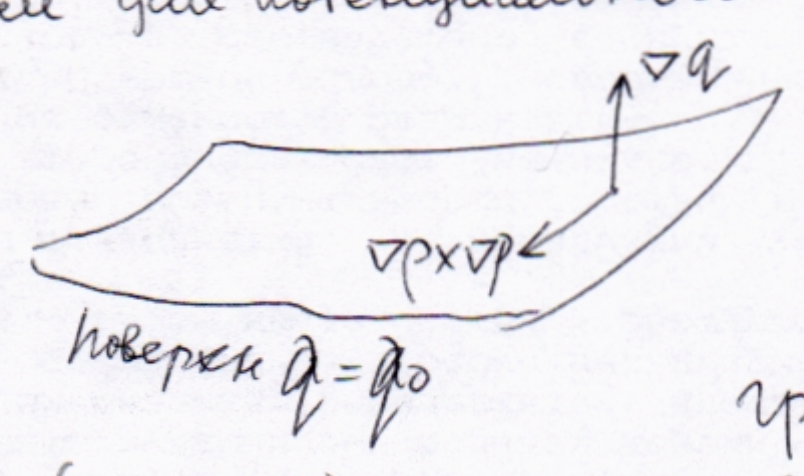
\includegraphics[width=0.5\linewidth]{pics/ch10.4.png}
    \caption{\label{fig:ch10.4}
    Ориентация $\nabla q$ по отношению к $\nabla\rho\times\nabla p$
    }
    \end{figure}    

Следует отметить, что в качестве $\sigma$ в уравнении (\ref{eq:ch10-temp}) может выступать любая величина, сохраняющаяся в частице: потенциальная температура в случае воздуха, температура или соленость в случае воды. Важно чтобы в недиссипативном случае удовлетворялось условие

\begin{equation}
    \label{eq:ch10-theta11}
    \td{S}{t}=0,
\end{equation}
где $S$ -- одна из указанных переменных.

Поскольку вращение Земли постоянно, то уравнения относительного вихря сохраняют свой форму и для абсолютного вихря $\vec{\Omega_a}=\vec{\Omega}+2\vec{\omega}$ и (при отсутствии диссипативных сил и источников) выражение для потенциального вихря примет вид

\begin{equation*}
    \td{}{t} \qb{ \frac{\vec{\Omega_a}\nabla\sigma}{\rho}  } = 0.
\end{equation*}

Если жидкость несжимаема, но стратифицирована, то сама плотность удовлетворяет условию \ref{eq:ch10-theta11}. В таком потоке справедливо условие

\begin{equation*}
    \td{}{t} \qb{ \frac{\vec{\Omega_a}\nabla p  }{\rho}  } = 0.
\end{equation*}

Как уже отмечалось выше, потенциальный вихрь представляет собой проекцию вектора вихря на градиент энтропии. Для большей обозримости физического смысла потенциального вихря рассмотрим частный случай с сохранением только вертикальной составляющей вихря скорости $\omega_z$, а вместо энтропии будем использовать потенциальную температуру, причемс сохраним в операторе градиента только градиент по вертикали. Последнее предположение вполне оправдано, поскольку в атмосфере $\pd{Q}{z}\gg\pd{Q}{x}, \pd{Q}{y}$. В этом случае потенциальный вихрь примет вид

\begin{equation}
    \label{eq:ch10-theta12}
    q_z = \frac{(\omega_z+l)\pd{Q}{z}}{\rho}.
\end{equation}
Из этого выражения видно, что большие положитель ные значения $q_z$ могут иметь в условиях одновременного существования циклонической завихренности и устойчивой стратификации, а отрицательные значения $q_z$ при антициклонической циркуляции воздуха или при сухонеустойчивой стратификации атмосферы, что бывает крайне редко за пределами пограничного слоя. Таким образом, потенциальный вихрь может служить, например, хорошим средством диагностики областей опускания стратосферного воздуха в высотных ложбинах циклона, давая в них большие значения $q_z$.

Поскольку в идеальной жидкости при отсутствии источников тепла потенциальный вихрь в частице сохраняется, в рассмотренном нами выше упрощенном варианте формулировки потенциального вихря (\ref{eq:ch10-theta12}) будем иметь

\begin{equation}
    \label{eq:ch10-theta13}
    \td{q_z}{t} = \td{}{t} \qb{ \frac{(\omega_z+l)\pd{\theta}{z} }{\rho} }.
\end{equation}
Из этого выражения следует, что если по какой-то причине вертикальный градиент потенциальной температуры начал убывать, то из условия сохранения потенциального вихря неизбежно должна увеличиваться относительная завихренность $\omega_z$, т.е. условия сохранения потенциального вихря в частице могут дать нам указание относительно эволюции одного из компонентов $q_z$ при известном изменении другого компонента.

\begin{warn}
    Дальше можно вставить кусок про потенциальную завихренность во влажной атмосфере, но я пока в ней не разобрался
\end{warn}











\section{Уравнение спиральности}

\section{Уравнение энергии}

\section{Уравнение дивергенции скорости}

\section{Уравнение тенденции}

